\section{Introduction}
In \cite{huberman_evolutionary_1993} the authors showed that the results of simulating the classic prisoners-dilemma game on a 2D-grid as reported in \cite{nowak_evolutionary_1992} depends on a a very specific strategy of iterating the simulation and show that the beautiful patterns seen in figure \ref{fig:sync_patterns} will not form when selecting a different update-strategy.

\begin{figure}[H]
	\centering
  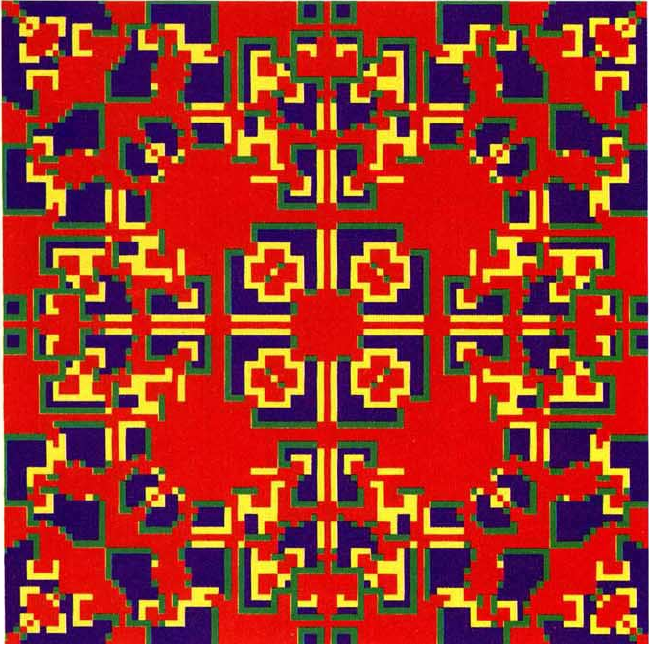
\includegraphics[width=.4\textwidth, angle=0]{./fig/sync_patterns.png}
	\caption{Patterns formed by playing the prisoners-dilemma game on a 2D-grid using a \textit{synchronous} update-strategy. Picture taken from \cite{huberman_evolutionary_1993}.}
	\label{fig:sync_patterns}
\end{figure}

Although the authors differentiated between two strategies, their description still lacks precision and detail. They also discussed philosophical aspects of choosing one strategy over the other, but lacked to generalize their observation. Thus we generalize their observation in our main message of this paper that \textit{when developing a model for an ABS it is of most importance to select the right update-strategy which reflects and supports the corresponding semantics of the model}. As we will show in the section on Related Research, we find that due to conflicting ideas about update-strategies this awareness is yet still under-represented in the field of ABS and is lacking a systematic treatment. Thus our contribution in this paper is to
\begin{itemize}
	\item Present general properties of ABS.
	\item Derive update-strategies from these properties.
	\item Establish a general terminology of talking about these update-strategies.
	\item Compare the three programming languages Java, Haskell and Scala with Actors in regard of their suitability to implement each of these strategies.
\end{itemize}

It is important to note that the amount of research on using Haskell in the field of ABS has so far been moderate. Though there exist a few papers which look into Haskell and ABS \cite{de_jong_suitability_2014}, \cite{sulzmann_specifying_2007}, \cite{jankovic_functional_2007} all treat Haskell in this context very generally and focus primarily on how to specify Agents. An interesting library for Discrete Event Simulation (DES) and System Dynamics (SD) in Haskell called \textit{Aivika 3} is described in \cite{sorokin_aivika_2015}. It also comes with very basic features for ABS but only allows to specify simple state-based Agents with timed transitions. Thus this papers is investigating Haskell in a more fundamental way by looking into its suitability in implementing update-strategies in ABS, something not looked at in the ABS community thus presenting an original novelty as well.